% !TeX program = xelatex
\documentclass[a4paper,10pt]{article}

% ============================================================================
% កិច្ចតែងការបង្រៀនមុខវិជ្ជាគណិតវិទ្យា ថ្នាក់ទី៨ (ម៉ោងសិក្សា ៥០ នាទី — គ្មាន LCD / ប្រើសន្លឹកកិច្ចការជាគោល)
% មេរៀនទី១៧៖ រូបធរណីមាត្រដែលមានវិមាត្របី | ម៉ោងទី៤ (១៧.២)៖ ការគណនាមាឌនៃព្រីស (ទំ.២២២–២២៣)
% វិធីសាស្ត្រ៖ 3-Layer Unit-Cube Spatial Structuring + Cross-Sectional Extrusion (V = B*h) & POE Overflow Worksheet
% ============================================================================
\usepackage[a4paper, left=0.95cm, right=0.95cm, top=0.85cm, bottom=0.92cm, footskip=0.52cm]{geometry}
\usepackage{amsmath}
\usepackage{unicode-math}
\usepackage{fontspec}
\usepackage{longtable, array, multirow, colortbl}
\usepackage[table]{xcolor}
\usepackage{enumitem}
\usepackage{pifont}
\usepackage{fancyhdr}
\usepackage{tikz}
\usetikzlibrary{calc, arrows.meta, angles, quotes, patterns, decorations.markings, babel}

\makeatletter
\let\@expl@@@mark@update@singlecol@structures@@\relax
\makeatother

% -------------------- ការស្វែងរកទីតាំងពុម្ពអក្សរដោយស្វ័យប្រវត្តិ (\NGSFindFonts) --------------------
\providecommand{\NGSFindFonts}{%
  \IfFileExists{C:/Windows/Fonts/cambria.ttc}{%
    \def\NGSSysPath{C:/Windows/Fonts/}%
    \def\NGSUserPath{C:/Users/KIT/AppData/Local/Microsoft/Windows/Fonts/}%
  }{%
    \IfFileExists{./fonts/KhmerOSsiemreap.ttf}{\def\NGSSysPath{./fonts/}\def\NGSUserPath{./fonts/}}{%
    \IfFileExists{../fonts/KhmerOSsiemreap.ttf}{\def\NGSSysPath{../fonts/}\def\NGSUserPath{../fonts/}}{%
    \IfFileExists{../../fonts/KhmerOSsiemreap.ttf}{\def\NGSSysPath{../../fonts/}\def\NGSUserPath{../../fonts/}}{%
    \IfFileExists{../../../fonts/KhmerOSsiemreap.ttf}{\def\NGSSysPath{../../../fonts/}\def\NGSUserPath{../../../fonts/}}{%
    \IfFileExists{../../../../fonts/KhmerOSsiemreap.ttf}{\def\NGSSysPath{../../../../fonts/}\def\NGSUserPath{../../../../fonts/}}{%
    \IfFileExists{../../../../../fonts/KhmerOSsiemreap.ttf}{\def\NGSSysPath{../../../../../fonts/}\def\NGSUserPath{../../../../../fonts/}}{%
    \IfFileExists{../../../../../../fonts/KhmerOSsiemreap.ttf}{\def\NGSSysPath{../../../../../../fonts/}\def\NGSUserPath{../../../../../../fonts/}}{%
      \def\NGSSysPath{../../../../../../../fonts/}\def\NGSUserPath{../../../../../../../fonts/}%
    }}}}}}}%
  }%
}
\NGSFindFonts

\setmathfont[Path={\NGSSysPath}, FontIndex=1, Scale=1.02]{cambria.ttc}
\defaultfontfeatures{Ligatures=TeX}

\setmainfont[
  Path={\NGSUserPath},
  Extension=.ttf,
  Script=Khmer,
  BoldFont={KhmerOSsiemreap},
  BoldFeatures={FakeBold=1.8},
  ItalicFont={KhmerOSsiemreap},
  ItalicFeatures={FakeSlant=0.25},
  BoldItalicFont={KhmerOSsiemreap},
  BoldItalicFeatures={FakeBold=1.8, FakeSlant=0.25}
]{KhmerOSsiemreap}

\newfontfamily\muol[
  Path={\NGSUserPath},
  Extension=.ttf,
  Script=Khmer
]{KhmerOSmuollight}

\newfontfamily\NagaBold[
  Path={\NGSUserPath},
  Extension=.ttf,
  Script=Khmer,
  ItalicFont={AKbalthom Naga Bold},
  ItalicFeatures={FakeSlant=0.22}
]{AKbalthom Naga Bold}

\newfontfamily\Tacteing[
  Path={\NGSUserPath},
  Extension=.TTF
]{TACTENG}

\newfontfamily\CalibriPage[
  Path={\NGSSysPath},
  Extension=.ttf
]{calibri}

\newfontfamily\TimesEn[
  Path={\NGSSysPath},
  Extension=.ttf,
  BoldFont={timesbd},
  ItalicFont={timesi},
  BoldItalicFont={timesbi}
]{times}

\newfontfamily\SymbolCirc[
  Path={\NGSSysPath},
  Extension=.ttf
]{cour}
\newcommand{\wcirc}{{\SymbolCirc\fontsize{10.5pt}{12pt}\selectfont o}}

\XeTeXlinebreaklocale "km"
\XeTeXlinebreakskip = 0pt plus 1pt minus 0.1pt

% -------------------- ពណ៌ និងការតុបតែង --------------------
\definecolor{darkred}{RGB}{180, 0, 0}
\definecolor{red5e}{RGB}{210, 15, 15}
\definecolor{headgray}{gray}{0.86}
\definecolor{stepgray}{gray}{0.91}
\definecolor{boxgray}{gray}{0.93}

\pagestyle{fancy}
\fancyhf{}
\renewcommand{\headrulewidth}{0pt}
\fancyfoot[R]{{\CalibriPage\fontsize{9.5pt}{11pt}\selectfont \thepage}}

\setlength{\parindent}{0pt}
\setlength{\parskip}{0pt}
\setlength{\LTpre}{2pt}
\setlength{\LTpost}{2pt}
\setlength{\tabcolsep}{4.5pt}
\arrayrulewidth=0.45pt

\newcolumntype{L}[1]{>{\raggedright\arraybackslash}p{#1}}
\newcolumntype{C}[1]{>{\centering\arraybackslash}p{#1}}

\newcommand{\en}[1]{{\TimesEn #1}}
\newcommand{\enbf}[1]{{\TimesEn\textbf{#1}}}
\newcommand{\unit}[1]{\,\text{\en{#1}}}
\newcommand{\fiveE}[1]{{\NagaBold\fontsize{9.5pt}{13pt}\selectfont\textcolor{red5e}{#1}}}
\newcommand{\timenote}[1]{\textcolor{darkred}{\textit{#1}}}
\newcommand{\khmflourish}{{\Tacteing\fontsize{17pt}{17pt}\selectfont 3}}
\newcommand{\graybox}[1]{\colorbox{boxgray}{\strut\hspace{2pt}#1\hspace{2pt}}}
\newcommand{\ditem}{\tikz[baseline=-0.5ex]\fill (0,0.42ex) -- (0.42ex,0) -- (0,-0.42ex) -- (-0.42ex,0) -- cycle;\hspace{0.3em}}
\newcommand{\cnum}[1]{{\fontsize{10.5pt}{12pt}\selectfont\ding{\numexpr181+#1\relax}}\hspace{0.2em}}
\newcommand{\cfig}[1]{\par\vspace{4pt}{\centering #1\par}\vspace{4pt}}
\newcommand{\stepheader}[1]{\multicolumn{3}{|c|}{\cellcolor{stepgray}\muol #1} \\* \noalign{\hrule height 0.4pt}}
\newcommand{\tri}[1]{\ensuremath{\triangle #1}}

\newcommand{\rightbox}[4][0.18]{%
  \draw[black, line width=0.75pt]
    ($(#3)!#1!(#2)$) -- ($($(#3)!#1!(#2)$)+($(#3)!#1!(#4)$)-(#3)$) -- ($(#3)!#1!(#4)$);
}

% ============================================================================
% រូបធរណីមាត្រ ស-ខ្មៅ (B&W Print-Safe TikZ Figures for Hour 17.4: Prism Volume)
% ============================================================================

% ១. កំណែកិច្ចការផ្ទះទី៦ (ទំ.២២៧) និងរំលឹកផ្ទៃបាតព្រីស/ស៊ីឡាំង
\newcommand{\figPrereqPrismVol}{%
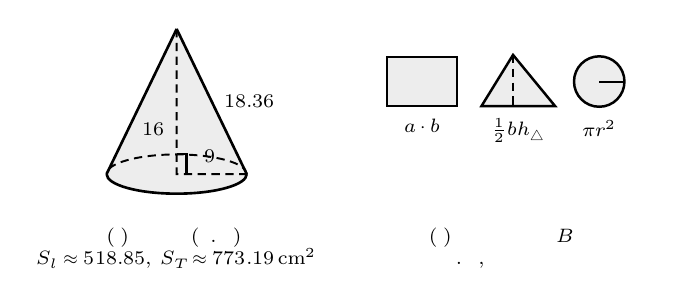
\begin{tikzpicture}[scale=0.89, every node/.style={font=\scriptsize, text=black}]
  % (ក) លំហាត់ទី៦ ទំ.២២៧៖ កោន r=9cm, h=16cm => s = sqrt(337) ~= 18.36cm
  \begin{scope}[shift={(-2.30,0)}]
    \coordinate (V) at (0,1.35);
    \coordinate (O) at (0,-0.72);
    \coordinate (L) at (-1.00,-0.72);
    \coordinate (R) at (1.00,-0.72);
    \fill[gray!14] (L) -- (V) -- (R) arc (0:-180:1.00 and 0.28);
    \draw[black, line width=0.95pt] (L) arc (-180:0:1.00 and 0.28) (V) -- (L) (V) -- (R);
    \draw[black, line width=0.7pt, densely dashed] (R) arc (0:180:1.00 and 0.28) (V) -- (O) -- (R);
    \rightbox[0.14]{V}{O}{R}
    \node[left=1pt] at (0,-0.08) {$16$};
    \node[above=0.5pt] at (0.48,-0.72) {$9$};
    \node[right=1pt] at ($0.5*(V)+0.5*(R)$) {$18.36$};
    \node[align=center, text width=3.55cm] at (0,-1.78) {(ក) លំហាត់ទី៦ (ទំ.២២៧)៖\\$S_l\approx 518.85,\; S_T\approx 773.19\unit{cm}^2$};
  \end{scope}

  % (ខ) រំលឹកផ្ទៃក្រឡាបាត B (ចតុ.កែង, ត្រីកោណ, ថាស)
  \begin{scope}[shift={(2.15,0.10)}]
    \draw[black, line width=0.9pt, fill=gray!14] (-1.45,0.15) rectangle (-0.45,0.85);
    \node[below=1pt] at (-0.95,0.15) {$a\cdot b$};
    \draw[black, line width=0.9pt, fill=gray!14] (-0.10,0.15) -- (0.95,0.15) -- (0.35,0.88) -- cycle;
    \draw[black, line width=0.65pt, densely dashed] (0.35,0.88) -- (0.35,0.15);
    \node[below=1pt] at (0.42,0.15) {$\frac{1}{2}bh_{\tri{}}$};
    \draw[black, line width=0.9pt, fill=gray!14] (1.58,0.50) circle (0.36cm);
    \draw[black, line width=0.7pt] (1.58,0.50) -- (1.94,0.50);
    \node[below=1pt] at (1.58,0.12) {$\pi r^2$};
    \node[align=center, text width=3.65cm] at (0.22,-1.88) {(ខ) រំលឹកផ្ទៃក្រឡាបាត $B$៖\\ចតុ.កែង, ត្រីកោណ និងថាស};
  \end{scope}
\end{tikzpicture}}

% ២. E1 Engage (លំហាត់ទី១៥ ទំ.២២៩)៖ ចាក់ទឹកពេញពែងស៊ីឡាំង (d=8cm, h=15cm) ចូលថាសប្រអប់កែង (15x10x5cm)
\newcommand{\figEngageOverflow}{%
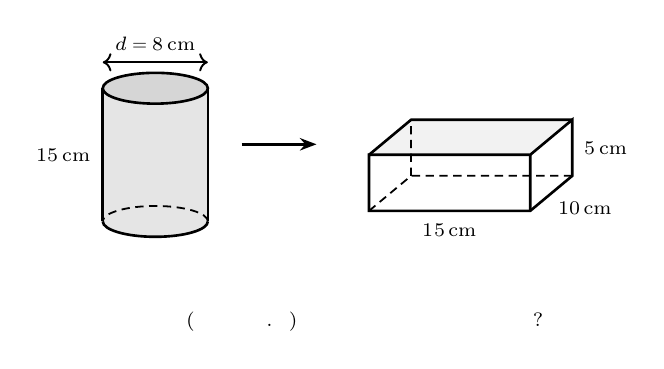
\begin{tikzpicture}[scale=0.89, every node/.style={font=\scriptsize, text=black}]
  % ពែងស៊ីឡាំងពេញទឹក (d=8 => r=4, h=15)
  \begin{scope}[shift={(-2.45,0)}]
    \fill[gray!20] (-0.75,-0.95) -- (-0.75,0.95) arc (180:360:0.75 and 0.22) -- (0.75,-0.95) arc (0:-180:0.75 and 0.22);
    \fill[gray!32] (0,0.95) ellipse (0.75 and 0.22);
    \draw[black, line width=0.95pt] (0,0.95) ellipse (0.75 and 0.22);
    \draw[black, line width=0.95pt] (-0.75,-0.95) -- (-0.75,0.95) (0.75,-0.95) -- (0.75,0.95);
    \draw[black, line width=0.95pt] (-0.75,-0.95) arc (-180:0:0.75 and 0.22);
    \draw[black, line width=0.65pt, densely dashed] (0.75,-0.95) arc (0:180:0.75 and 0.22);
    \draw[<->, line width=0.7pt] (-0.75,1.32) -- (0.75,1.32) node[midway, above=0.5pt] {$d=8\unit{cm}$};
    \node[left=1pt] at (-0.75,0) {$15\unit{cm}$};
    \node at (0,-1.52) {\textbf{ពែងស៊ីឡាំងពេញទឹក}};
  \end{scope}

  \draw[-{Stealth[length=2.1mm]}, line width=0.95pt] (-1.22,0.15) -- (-0.15,0.15) node[midway, above=1pt] {ចាក់ទឹកចូល};

  % ថាសប្រអប់កែង 15 x 10 x 5 cm
  \begin{scope}[shift={(2.05,-0.15)}]
    \coordinate (A) at (-1.45,-0.65);
    \coordinate (B) at (0.85,-0.65);
    \coordinate (C) at (1.45,-0.15);
    \coordinate (D) at (-0.85,-0.15);
    \coordinate (A1) at (-1.45,0.15);
    \coordinate (B1) at (0.85,0.15);
    \coordinate (C1) at (1.45,0.65);
    \coordinate (D1) at (-0.85,0.65);
    \fill[gray!10] (A1) -- (B1) -- (C1) -- (D1) -- cycle;
    \draw[black, line width=0.95pt] (A) -- (B) -- (C) -- (C1) -- (B1) -- (A1) -- cycle;
    \draw[black, line width=0.95pt] (A1) -- (D1) -- (C1) (B) -- (B1);
    \draw[black, line width=0.65pt, densely dashed] (A) -- (D) -- (C) (D) -- (D1);
    \node[below=1pt] at (-0.30,-0.65) {$15\unit{cm}$};
    \node[below right=-1pt] at (1.15,-0.42) {$10\unit{cm}$};
    \node[right=1pt] at (1.45,0.25) {$5\unit{cm}$};
    \node at (0.0,-1.37) {\textbf{ថាសប្រអប់កែងទទេ}};
  \end{scope}

  \node[align=center, text width=7.2cm] at (-0.05,-2.38) {បញ្ហាជាក់ស្ដែង (លំហាត់ទី១៥ ទំ.២២៩)៖ ពេលចាក់ទឹកពេញពែងចូលថាស តើទឹកហៀរចេញក្រៅឬទេ?};
\end{tikzpicture}}

% ៣. E2/E3 ការតម្រៀបគូបឯកតា ៣ ស្រទាប់ (4x2x3 = 24 cm^3, ទំ.២២២) និងលំហាត់គំរូទី 2 (ព្រីសត្រីកោណសមបាទ 10,10,12 ប្រវែង 15, ទំ.២២៣)
\newcommand{\figLayerAndTriPrism}{%
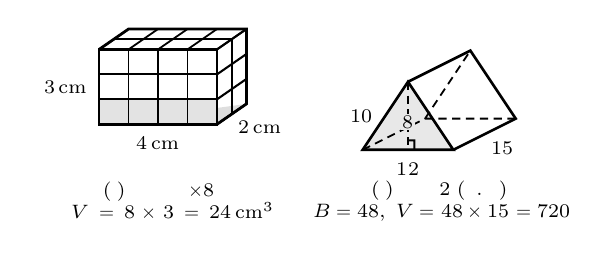
\begin{tikzpicture}[scale=0.72, every node/.style={font=\scriptsize, text=black}]
  % (ក) ប្រអប់កែង 4 x 2 x 3 cm បំបែកជា 3 ស្រទាប់ (8 គូបក្នុង 1 ស្រទាប់)
  \begin{scope}[shift={(-3.65,-0.15)}]
    \def\ux{0.52}
    \def\uy{0.44}
    \def\sx{0.26}
    \def\sy{0.18}
    \fill[gray!26] (0,0) -- (4*\ux,0) -- ($(4*\ux,0)+(2*\sx,2*\sy)$) -- ($(0,\uy)+(2*\sx,2*\sy)+(4*\ux,0)-(0,\uy)$) -- cycle;
    \fill[gray!22] (0,0) rectangle (4*\ux,\uy);
    \foreach \x in {0,1,2,3,4} {
      \draw[black, line width=0.65pt] (\x*\ux,0) -- (\x*\ux,3*\uy);
    }
    \foreach \y in {0,1,2,3} {
      \draw[black, line width=0.75pt] (0,\y*\uy) -- (4*\ux,\y*\uy);
    }
    \foreach \x in {0,1,2,3,4} {
      \draw[black, line width=0.65pt] (\x*\ux,3*\uy) -- ($(\x*\ux,3*\uy)+(2*\sx,2*\sy)$);
    }
    \foreach \z in {0,1,2} {
      \draw[black, line width=0.65pt] ($(\z*\sx,3*\uy+\z*\sy)$) -- ($(4*\ux+\z*\sx,3*\uy+\z*\sy)$);
    }
    \foreach \z in {0,1,2} {
      \draw[black, line width=0.65pt] ($(4*\ux+\z*\sx,\z*\sy)$) -- ($(4*\ux+\z*\sx,3*\uy+\z*\sy)$);
    }
    \foreach \y in {0,1,2,3} {
      \draw[black, line width=0.75pt] (4*\ux,\y*\uy) -- ($(4*\ux+2*\sx,\y*\uy+2*\sy)$);
    }
    \draw[black, line width=1.0pt] (0,0) rectangle (4*\ux,3*\uy);
    \draw[black, line width=1.0pt] (0,3*\uy) -- ($(2*\sx,3*\uy+2*\sy)$) -- ($(4*\ux+2*\sx,3*\uy+2*\sy)$) -- ($(4*\ux+2*\sx,2*\sy)$) -- (4*\ux,0);
    \node[below=1pt] at (2*\ux,0) {$4\unit{cm}$};
    \node[below right=-1pt] at ($(4*\ux+\sx,\sy)$) {$2\unit{cm}$};
    \node[left=1pt] at (0,1.5*\uy) {$3\unit{cm}$};
    \node[align=center, text width=3.45cm] at (1.30,-1.35) {(ក) ៣ ស្រទាប់ $\times 8$ គូប៖\\$V = 8\times 3 = 24\unit{cm}^3$};
  \end{scope}

  % (ខ) លំហាត់គំរូទី 2 ទំ.២២៣៖ ព្រីសត្រីកោណសមបាទ (10,10,12) ប្រវែង h=15
  \begin{scope}[shift={(2.35,0.05)}]
    \coordinate (P1) at (-1.35,-0.65);
    \coordinate (P2) at (0.25,-0.65);
    \coordinate (P3) at (-0.55,0.55);
    \coordinate (M) at (-0.55,-0.65);
    \coordinate (Q1) at (-0.25,-0.10);
    \coordinate (Q2) at (1.35,-0.10);
    \coordinate (Q3) at (0.55,1.10);
    \fill[gray!18] (P1) -- (P2) -- (P3) -- cycle;
    \draw[black, line width=0.95pt] (P1) -- (P2) -- (P3) -- cycle;
    \draw[black, line width=0.95pt] (P2) -- (Q2) -- (Q3) -- (P3);
    \draw[black, line width=0.65pt, densely dashed] (P1) -- (Q1) -- (Q2) (Q1) -- (Q3);
    \draw[black, line width=0.75pt, densely dashed] (P3) -- (M);
    \rightbox[0.14]{P3}{M}{P2}
    \node[below=1pt] at (-0.55,-0.65) {$12$};
    \node[left=1pt] at ($0.5*(P1)+0.5*(P3)$) {$10$};
    \node[fill=gray!18, inner sep=0.6pt] at (-0.55,-0.16) {$8$};
    \node[below right=-1pt] at ($0.5*(P2)+0.5*(Q2)$) {$15$};
    \node[align=center, text width=3.45cm] at (0.05,-1.55) {(ខ) គំរូទី \en{2} (ទំ.២២៣)៖\\$B=48,\; V=48\times 15=720$};
  \end{scope}
\end{tikzpicture}}

% ៤. E4 ប្រតិបត្តិ ក (4x7x5 mm) និង ប្រតិបត្តិ ខ (ព្រីសត្រីកោណកែង 8m, 12m, ប្រវែង 16m) ទំ.២២៣
\newcommand{\figElaboratePrismVol}{%
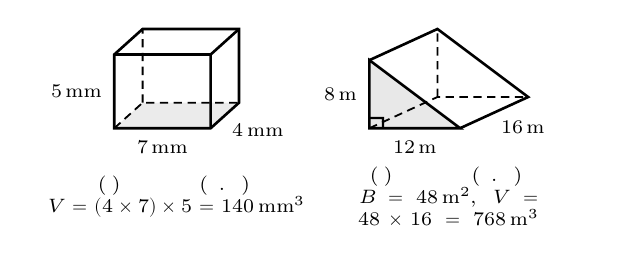
\begin{tikzpicture}[scale=0.72, every node/.style={font=\scriptsize, text=black}]
  % (១) ប្រតិបត្តិ ក (ទំ.២២៣)៖ ប្រអប់កែង 4mm x 7mm x 5mm
  \begin{scope}[shift={(-2.35,0)}]
    \coordinate (A) at (-1.15,-0.65);
    \coordinate (B) at (0.55,-0.65);
    \coordinate (C) at (1.05,-0.20);
    \coordinate (D) at (-0.65,-0.20);
    \coordinate (A1) at (-1.15,0.65);
    \coordinate (B1) at (0.55,0.65);
    \coordinate (C1) at (1.05,1.10);
    \coordinate (D1) at (-0.65,1.10);
    \fill[gray!16] (A) -- (B) -- (C) -- (D) -- cycle;
    \draw[black, line width=0.95pt] (A) -- (B) -- (C) -- (C1) -- (D1) -- (A1) -- cycle;
    \draw[black, line width=0.95pt] (A1) -- (B1) -- (C1) (B) -- (B1);
    \draw[black, line width=0.65pt, densely dashed] (A) -- (D) -- (C) (D) -- (D1);
    \node[below=1pt] at (-0.30,-0.65) {$7\unit{mm}$};
    \node[below right=-1pt] at (0.82,-0.45) {$4\unit{mm}$};
    \node[left=1pt] at (-1.15,0.0) {$5\unit{mm}$};
    \node[align=center, text width=3.55cm] at (-0.05,-1.85) {(១) ប្រតិបត្តិ ក (ទំ.២២៣)៖\\$V = (4\times 7)\times 5 = 140\unit{mm}^3$};
  \end{scope}

  % (២) ប្រតិបត្តិ ខ (ទំ.២២៣)៖ ព្រីសត្រីកោណកែង ជើង 8m, 12m និងប្រវែងព្រីស 16m
  \begin{scope}[shift={(2.35,0)}]
    \coordinate (A) at (-1.35,-0.65);
    \coordinate (B) at (0.25,-0.65);
    \coordinate (C) at (-1.35,0.55);
    \coordinate (A2) at (-0.15,-0.10);
    \coordinate (B2) at (1.45,-0.10);
    \coordinate (C2) at (-0.15,1.10);
    \fill[gray!18] (A) -- (B) -- (C) -- cycle;
    \draw[black, line width=0.95pt] (A) -- (B) -- (C) -- cycle;
    \draw[black, line width=0.95pt] (B) -- (B2) -- (C2) -- (C);
    \draw[black, line width=0.65pt, densely dashed] (A) -- (A2) -- (B2) (A2) -- (C2);
    \rightbox[0.15]{C}{A}{B}
    \node[left=1pt] at (-1.35,-0.05) {$8\unit{m}$};
    \node[below=1pt] at (-0.55,-0.65) {$12\unit{m}$};
    \node[below right=-1pt] at (0.85,-0.40) {$16\unit{m}$};
    \node[align=center, text width=3.65cm] at (0.05,-1.85) {(២) ប្រតិបត្តិ ខ (ទំ.២២៣)៖\\$B=48\unit{m}^2,\; V=48\times 16=768\unit{m}^3$};
  \end{scope}
\end{tikzpicture}}

% ============================================================================
% ចាប់ផ្ដើមឯកសារ (Document Body)
% ============================================================================
\begin{document}
\fontsize{10pt}{15.2pt}\selectfont

% -------------------- ក្បាលកិច្ចតែងការ (Header) --------------------
\begin{center}
  {\muol\fontsize{11pt}{16pt}\selectfont ព្រះរាជាណាចក្រកម្ពុជា}\\[2pt]
  {\muol\fontsize{10pt}{15pt}\selectfont ជាតិ សាសនា ព្រះមហាក្សត្រ}\\[1pt]
  \khmflourish
\end{center}

\vspace{-26pt}
{\muol\fontsize{9.5pt}{12.8pt}\selectfont
មន្ទីរអប់រំ យុវជន និងកីឡា ខេត្តកំពង់ធំ\\
ការិយាល័យអប់រំ យុវជន និងកីឡា ស្រុកកំពង់ស្វាយ\\
អនុវិទ្យាល័យព្រះក្រសាំង}

\vspace{1pt}
\begin{center}
  {\muol\fontsize{10pt}{14.5pt}\selectfont កិច្ចតែងការបង្រៀន}
\end{center}
\vspace{0pt}

% -------------------- ព័ត៌មានទូទៅ (Metadata) --------------------
{\renewcommand{\arraystretch}{0.98}
\hspace*{4.05cm}%
\begin{tabular}{@{}l l l@{}}
  - \hspace{0.35cm} មុខវិជ្ជា & : & គណិតវិទ្យា ថ្នាក់ទី៨ \\
  - \hspace{0.35cm} ចំណងជើងមេរៀន & : & មេរៀនទី១៧ រូបធរណីមាត្រដែលមានវិមាត្របី \\
  - \hspace{0.35cm} ចំណងជើងរង & : & ១៧.២ ការគណនាមាឌនៃព្រីស (ទំព័រ ២២២--២២៣) \\
  - \hspace{0.35cm} រយៈពេល & : & ១ ម៉ោងសិក្សា (៥០ នាទី) \\
  - \hspace{0.35cm} បង្រៀនដោយ & : & ហុក ប៊ុនថែន \\
  - \hspace{0.35cm} កាលបរិច្ឆេទ & : & ថ្ងៃ\makebox[18mm]{\dotfill}\ ទី\makebox[8mm]{\dotfill}\ ខែ\makebox[18mm]{\dotfill}\ ឆ្នាំ២០២៦ \\
\end{tabular}

\vspace{2pt}

% -------------------- I. វត្ថុបំណង --------------------
\textbf{I.} {\muol វត្ថុបំណង}\\[1pt]
\hspace*{0.55cm}%
\begin{tabular}{@{}l l L{14.2cm}@{}}
  \wcirc \hspace{0.25cm} វិជ្ជាសម្បទា & : & សិស្សប្រាប់បានត្រឹមត្រូវពីអត្ថន័យនៃមាឌតាមរយៈចំនួនគូបឯកតា ខ្នាតមាឌ ($\unit{mm}^3, \unit{cm}^3, \unit{dm}^3, \unit{m}^3$) និងរូបមន្តមាឌនៃព្រីសទូទៅ ($V = B \cdot h$) ព្រមទាំងប្រអប់កែង ($V = a \cdot b \cdot h$) និងស៊ីឡាំង ($V = \pi r^2 h$) ។ \\
  \wcirc \hspace{0.25cm} បំណិនសម្បទា & : & សិស្សកំណត់មុខបាត $B$ និងកម្ពស់កែង $h$ បានត្រឹមត្រូវ (ទោះបីព្រីសដេកផ្ដេកក៏ដោយ) រួចគណនាមាឌនៃព្រីសចតុមុខ ព្រីសត្រីមុខ និងស៊ីឡាំងលើសន្លឹកកិច្ចការ ព្រមទាំងដោះស្រាយបញ្ហាប្រៀបធៀបចំណុះទឹកជាក់ស្ដែង ។ \\
  \wcirc \hspace{0.25cm} ចរិយាសម្បទា & : & សិស្សមានភាពម៉ត់ចត់ក្នុងការពិនិត្យមុខបាតស្របប៉ុនគ្នាទាំងពីរ និងសរសេរខ្នាតគូបឱ្យត្រូវតាមទិន្នន័យនៃបញ្ហាជីវភាពរស់នៅ ។ \\
\end{tabular}

\vspace{2pt}

% -------------------- II. សម្ភារៈឧបទេស --------------------
\textbf{II.} {\muol សម្ភារៈឧបទេស}\\[1pt]
\hspace*{0.55cm}$\bullet$ \hspace{0.35cm} សៀវភៅសិក្សាគោលគណិតវិទ្យាថ្នាក់ទី៨ (ទំ.២២២--២២៣ និង ២២៨--២២៩) សន្លឹកកិច្ចការសិស្ស ស-ខ្មៅ (\en{Worksheet\_PRISM\_VOL} ចំនួន ២ ទំព័រ គ្មាន \en{LCD}) ក្ដារខៀន ដីស និងបន្ទាត់ក្រិត ។

\vspace{2pt}

% -------------------- III. វិធីសាស្រ្តបង្រៀន --------------------
\textbf{III.} {\muol វិធីសាស្រ្តបង្រៀន}\\[1pt]
\hspace*{0.45cm}%
\begin{tabular}{@{}l l L{14.85cm}@{}}
  $\bullet$ \hspace{0.25cm} គោលវិធី & : & សិស្សមជ្ឈមណ្ឌល (សិក្សាតាមរយៈការបំពេញលើសន្លឹកកិច្ចការជាគោល គ្មាន \en{LCD} និងគ្មានការកាត់បិទក្រដាស) \\
  $\bullet$ \hspace{0.25cm} យុទ្ធវិធីបង្រៀន & : & ស្ថាបនានិយម គម្រូ \en{5Es} រួមបញ្ចូលការរាប់ស្រទាប់គូបឯកតា (\en{3-Layer Unit-Cube Structuring}) ការទាញរូបមន្តតាមមុខកាត់បាត (\en{Cross-Sectional Extrusion} $V=B\cdot h$) និងការទស្សន៍ទាយ \en{POE} ។ \\
\end{tabular}
}

\vspace{2pt}

% -------------------- IV. ដំណើរការបង្រៀន --------------------
\textbf{IV.} {\muol ដំណើរការបង្រៀន}

\vspace{1pt}

\renewcommand{\arraystretch}{1.15}
\begin{longtable}{|L{5.50cm}|L{7.90cm}|L{4.80cm}|}
\hline
\rowcolor{headgray}
\multicolumn{1}{|c|}{\muol សកម្មភាពគ្រូ} &
\multicolumn{1}{c|}{\muol ខ្លឹមសារមេរៀន} &
\multicolumn{1}{c|}{\muol សកម្មភាពសិស្ស} \\
\hline
\endfirsthead

\hline
\rowcolor{headgray}
\multicolumn{1}{|c|}{\muol សកម្មភាពគ្រូ} &
\multicolumn{1}{c|}{\muol ខ្លឹមសារមេរៀន} &
\multicolumn{1}{c|}{\muol សកម្មភាពសិស្ស} \\
\hline
\endhead

\hline
\endfoot

\hline
\endlastfoot

% ==================== ជំហានទី១ (2 min) ====================
\stepheader{ជំហានទី១ (រដ្ឋបាលថ្នាក់)}
$\bullet$ ពិនិត្យវត្តមាន សណ្ដាប់ធ្នាប់ អនាម័យ និងចែកសន្លឹកកិច្ចការ \en{Worksheet\_PRISM\_VOL} ដល់សិស្សគ្រប់គូ \timenote{(2 min)}
&
$\bullet$ រដ្ឋបាលថ្នាក់ និងការត្រៀមសៀវភៅគោល បន្ទាត់ក្រិត និងសន្លឹកកិច្ចការសិស្ស
&
$\circ$ ប្រធានថ្នាក់រាយការណ៍វត្តមាន\par\vspace{2pt}
$\circ$ ទទួលសន្លឹកកិច្ចការ និងត្រៀមឧបករណ៍ \\[3pt]
\hline

% ==================== ជំហានទី២ (9 min: ≤3 + 3 + E1 3) ====================
\stepheader{ជំហានទី២ (កិច្ចការផ្ទះ + រំលឹកមេរៀនចាស់ + ទំនាក់ទំនងមេរៀនថ្មី)}
\timenote{(កំណែកិច្ចការផ្ទះ $\le 3\text{ min}$)}\par\vspace{1pt}
$\bullet$ ពិនិត្យចម្លើយលំហាត់ទី៦ (ទំ.២២៧) និងទី១២ (ទំ.២២៩) លើក្ដារខៀនយ៉ាងរហ័ស
&
\textbf{កំណែកិច្ចការផ្ទះ (ទំ.២២៧ ទី៦ និងទំ.២២៩ ទី១២)៖}\par\vspace{1pt}
$1.$ \textbf{ទី៦៖} $s = \sqrt{16^2+9^2} = \sqrt{337} \approx 18.36\unit{cm} \Rightarrow S_l \approx 518.85\unit{cm}^2$,\; $S_T \approx 518.85 + 254.34 = \mathbf{773.19\unit{cm}^2}$ ។\par\vspace{1pt}
$2.$ \textbf{ទី១២៖} $B = \pi r^2 = 160 \Rightarrow r \approx 7.14\unit{cm} \Rightarrow S_T = 160 + 3.142(7.14)(12) \approx \graybox{$429.21\unit{cm}^2$}$ ។
&
$\circ$ ផ្ទៀងផ្ទាត់និងកែកំណែលំហាត់ទី៦ និងទី១២ ក្នុងសៀវភៅ \\[3pt]

\timenote{(រំលឹកមេរៀនចាស់ 3 min)}\par\vspace{1pt}
$\bullet$ សួរ៖ «តើមុខបាតទាំងពីររបស់ព្រីសមានលក្ខណៈដូចម្ដេច? ចូររំលឹករូបមន្តផ្ទៃក្រឡាចតុ.កែង ត្រីកោណ និងថាស!»
&
\textbf{រំលឹកមុខបាតព្រីស និងរូបមន្តផ្ទៃក្រឡាបាត $B$៖}\par\vspace{1pt}
\ditem មុខបាតទាំងពីររបស់ព្រីសជាពហុកោណ \textbf{ប៉ុនគ្នា និងស្ថិតក្នុងប្លង់ស្របគ្នា} ។\par\vspace{1pt}
\ditem ចតុ.កែង៖ $B = a\cdot b$ \;\textbar\; ត្រីកោណ៖ $B = \frac{1}{2}bh_{\tri{}}$ \;\textbar\; ថាស៖ $B = \pi r^2$ ។
&
$\circ$ ឆ្លើយរំលឹកលក្ខណៈបាតព្រីស និងរូបមន្តផ្ទៃក្រឡាបាតទាំង ៣ \\[3pt]

& \cfig{\figPrereqPrismVol} & \\[3pt]

\fiveE{E1 - Engage} \timenote{(3 min)}\par\vspace{1.5pt}
$\bullet$ បង្ហាញបញ្ហាប្រៀបធៀបចំណុះទឹកលើ \textbf{បេសកកម្មទី១ (\en{E1})} (ដកស្រង់ពីលំហាត់ទី១៥ ទំ.២២៩)៖\par\vspace{1pt}
\hspace*{0.3em}-- «គេដងទឹកពេញពែងរាងស៊ីឡាំងមានអង្កត់ផ្ចិតបាត $8\unit{cm}$ និងកម្ពស់ $15\unit{cm}$ រួចចាក់ទឹកនោះទាំងអស់ចូលទៅក្នុងថាសប្រអប់កែងទទេមួយទំហំ $15\unit{cm}\times 10\unit{cm}\times 5\unit{cm}$ ។ តើទឹកនឹងហៀរចេញក្រៅថាស ឬអត់?»
&
\textbf{១៧.២ ការគណនាមាឌនៃព្រីស}\par\vspace{1.5pt}
\ditem \textbf{បញ្ហាបំផុសគំនិត (\en{E1 - POE})៖} ដើម្បីដឹងថាទឹកហៀរ ឬមិនហៀរ យើងត្រូវគណនា \textbf{មាឌ} (ចំណុះលំហខាងក្នុង) នៃពែងស៊ីឡាំង និងថាសប្រអប់កែង!
&
$\circ$ អានបេសកកម្មទី១ ពិភាក្សាជាដៃគូ និងគូសធីកទស្សន៍ទាយ (\en{Predict}) \\[3pt]

& \cfig{\figEngageOverflow} & \\[3pt]
\hline

% ==================== ជំហានទី៣ (17 min: E2 11 + E3 6) ====================
\stepheader{ជំហានទី៣ (ខ្លឹមសារមេរៀនថ្មី)}
\fiveE{E2 - Explore} \timenote{(11 min: 5 min)}\par\vspace{1pt}
$\bullet$ ឱ្យសិស្សធ្វើជាដៃគូលើ \textbf{ផ្នែកទី១ (ក) ការរាប់ស្រទាប់គូបឯកតា} តាមសៀវភៅទំ.២២២ (ប្រអប់កែងទំហំ $4\unit{cm}\times 2\unit{cm}\times 3\unit{cm}$)
&
\textbf{សកម្មភាពរុករកទី១ (ស្រទាប់គូបឯកតា $1\unit{cm}^3$)៖}\par\vspace{1pt}
$1.$ ស្រទាប់បាត ១ មានគូបឯកតាចំនួន $4\times 2 = \mathbf{8}$ គូប (ស្មើតម្លៃលេខនៃផ្ទៃក្រឡាបាត $B = 8\unit{cm}^2$) ។\par\vspace{1pt}
$2.$ បន្តុប $h = 3$ ស្រទាប់លើគ្នា $\Rightarrow$ សរុប $8\times 3 = \mathbf{24}$ គូបឯកតា ($24\unit{cm}^3$) ។
&
$\circ$ រាប់ចំនួនគូបក្នុង ១ ស្រទាប់ និងក្នុង ៣ ស្រទាប់លើសន្លឹកកិច្ចការ \\[3pt]

$\bullet$ ដើរសួរ៖ «ចុះបើបាតព្រីសជាត្រីកោណ ឬបញ្ចកោណមានផ្ទៃក្រឡា $B$ ហើយកម្ពស់ព្រីសគឺ $h$ តើមាឌ $V$ ស្មើនឹងអ្វី?»
&
$3.$ ជាទូទៅ ចំពោះគ្រប់ព្រីសត្រង់ (ត្រីមុខ ចតុមុខ បញ្ចមុខ និងស៊ីឡាំង)៖\par\vspace{1pt}
\hspace*{0.3em}មាឌ $=$ ផ្ទៃក្រឡាបាត $\times$ កម្ពស់ $\Rightarrow$ \graybox{$V = B \cdot h$} ។
&
$\circ$ ទាញបានរូបមន្តទូទៅ $V = B \cdot h$ \\[3pt]

\timenote{(E2 ទី២៖ លំហាត់គំរូទី \en{1} និងទី \en{2} ទំ.២២៣ — 6 min)}\par\vspace{1.5pt}
$\bullet$ ដឹកនាំសិស្សបំពេញ \textbf{ផ្នែកទី១ (ខ) គំរូទី \en{1}} (ប្រអប់កែង $20\times 5\times 15$) និង \textbf{គំរូទី \en{2}} (ព្រីសត្រីកោណដេកផ្ដេក) តាមទំ.២២៣
&
\textbf{សកម្មភាពរុករកទី២ — លំហាត់គំរូទី \en{1} និងទី \en{2} (ទំ.២២៣)៖}\par\vspace{1.5pt}
$\bullet$ \textbf{គំរូទី \en{1} (ប្រអប់កែង $20\times 5\times 15$)៖}\par\vspace{1pt}
\hspace*{0.2em}ផ្ទៃបាត $B = 20\times 5 = 100$;\; កម្ពស់ $h = 15 \Rightarrow V = 100\times 15 = \mathbf{1500}$ ឯកតាមាឌ ។\par\vspace{1.5pt}
$\bullet$ \textbf{គំរូទី \en{2} (ព្រីសត្រីកោណសមបាទ $10, 10, 12$ ប្រវែង $15$)៖}\par\vspace{1pt}
\hspace*{0.2em}កម្ពស់បាតត្រីកោណ $h_{\tri{}} = \sqrt{10^2-6^2} = 8 \Rightarrow B = \frac{1}{2}(12)(8) = 48$;\par\vspace{1pt}
\hspace*{0.2em}មាឌព្រីស៖ $V = B\cdot h = 48\times 15 = \graybox{$720$}$ ឯកតាមាឌ ។\par\vspace{1.5pt}
\ditem \textit{សម្គាល់៖ ទោះព្រីសដេកផ្ដេក ក៏បាត $B$ នៅតែជាត្រីកោណទាំងពីរដដែល!}
&
$\circ$ គណនាគំរូទី \en{1} បាន $V=1500$\par\vspace{2pt}
$\circ$ កំណត់បាតត្រីកោណនៃគំរូទី \en{2} រក $h_{\tri{}}=8, B=48$ រួចគណនា $V=720$ \\[3pt]

& \cfig{\figLayerAndTriPrism} & \\[3pt]

\fiveE{E3 - Explain} \timenote{(6 min)}\par\vspace{1.5pt}
$\bullet$ ហៅតំណាងគូបង្ហាញ រួចគ្រូសង្ខេបរូបមន្តមាឌព្រីស (ប្រអប់ទំ.២២២) ឱ្យសិស្សបំពេញ \textbf{ផ្នែកទី២}
&
\textbf{រូបមន្តមាឌនៃព្រីស និងស៊ីឡាំង (ទំ.២២២)៖}\par\vspace{1.5pt}
$\bullet$ មាឌនៃព្រីសស្មើនឹងផលគុណរវាងផ្ទៃក្រឡាបាត ($B$) និងកម្ពស់ ($h$)៖ \graybox{$V = B \cdot h$}\par\vspace{1.5pt}
\hspace*{0.2em}\ditem ប្រអប់កែង៖ $V = a\cdot b\cdot h$ \;\textbar\; គូប៖ $V = a^3$ \;\textbar\; ស៊ីឡាំង៖ $V = \pi r^2 h$ ។
&
$\circ$ តំណាងគូឡើងបកស្រាយ\par\vspace{2pt}
$\circ$ បំពេញប្រអប់រូបមន្តក្នុងផ្នែកទី២ \\[3pt]

$\bullet$ សង្កត់ធ្ងន់លើអន្ទាក់ «ព្រីសដេកផ្ដេក» ខ្នាតគូប និងធនាគារហេតុផល \cnum{1}--\cnum{4}
&
\textbf{ចំណុចប្រុងប្រយ័ត្ន និងធនាគារហេតុផល៖}\par\vspace{1.5pt}
$\bullet$ \cnum{1} មុខបាត $B$ គឺជាមុខពហុកោណពីរដែលប៉ុនគ្នានិងស្របគ្នា (មិនមែនមុខដែលដាក់ផ្ទាល់ដីជានិច្ចទេ!) \;\textbar\; \cnum{2} $h$ ជាចម្ងាយកែងរវាងបាតទាំងពីរ \;\textbar\; \cnum{3} $V = B\cdot h$ \;\textbar\; \cnum{4} ខ្នាតមាឌជាគូប ($1\unit{dm}^3 = 1\unit{L} = 1000\unit{cm}^3$) ។
&
$\circ$ កត់ចំណាំរបៀបសម្គាល់បាត $B$ ពេលព្រីសដេកផ្ដេក និងធនាគារហេតុផល \\[3pt]
\hline

% ==================== ជំហានទី៤ (20 min: E4 10 + E5 10) ====================
\stepheader{ជំហានទី៤ (ពង្រីកចំណេះដឹង និងវាយតម្លៃ)}
\fiveE{E4 - Elaborate} \timenote{(10 min: 4 min)}\par\vspace{1pt}
$\bullet$ ឱ្យសិស្សធ្វើជាដៃគូលើ \textbf{ផ្នែកទី៣ (ក) ប្រតិបត្តិ ក (ទំ.២២៣)} សម្រាប់ព្រីសចតុមុខកែង $4\unit{mm}\times 7\unit{mm}\times 5\unit{mm}$
&
\textbf{៣.ក ប្រតិបត្តិ ក (ទំ.២២៣ — ព្រីសចតុមុខកែង $4\unit{mm}\times 7\unit{mm}\times 5\unit{mm}$)៖}\par\vspace{1.5pt}
$\bullet$ ផ្ទៃក្រឡាបាត៖ $B = 4\times 7 = \mathbf{28\unit{mm}^2}$ ហើយកម្ពស់ $h = 5\unit{mm}$ ។\par\vspace{1pt}
$\bullet$ មាឌព្រីស៖ $V = B\cdot h = 28\times 5 = \graybox{$140\unit{mm}^3$}$ \cnum{3}\cnum{4} ។
&
$\circ$ គណនាផ្ទៃបាត $B=28\unit{mm}^2$ និងមាឌ $V=140\unit{mm}^3$ \\[3pt]

\timenote{(E4 ទី២៖ ប្រតិបត្តិ ខ ទំ.២២៣ — 6 min)}\par\vspace{1.5pt}
$\bullet$ ឱ្យសិស្សដោះស្រាយ \textbf{ផ្នែកទី៣ (ខ) ប្រតិបត្តិ ខ (ទំ.២២៣)} រួចសួរ \en{EIA Looking-Back}៖ «ហេតុអ្វីយើងមិនយកមុខក្រោម $12\unit{m}\times 16\unit{m}$ ធ្វើជាបាត $B$?»
&
\textbf{៣.ខ ប្រតិបត្តិ ខ (ទំ.២២៣ — ព្រីសត្រីកោណកែងដេកផ្ដេក)៖}\par\vspace{1.5pt}
$\bullet$ មុខបាតជាត្រីកោណកែងជើង $8\unit{m}$ និង $12\unit{m}$ \cnum{1}៖ $B = \frac{1}{2}\times 8\times 12 = \mathbf{48\unit{m}^2}$ ។\par\vspace{1pt}
$\bullet$ ចម្ងាយកែងរវាងបាតត្រីកោណទាំងពីរគឺ $h = 16\unit{m}$ \cnum{2} $\Rightarrow V = 48\times 16 = \graybox{$768\unit{m}^3$}$ ។
&
$\circ$ សម្គាល់បាតត្រីកោណកែង រក $B=48\unit{m}^2$ និងគណនា $V=768\unit{m}^3$ \\[3pt]

& \cfig{\figElaboratePrismVol} & \\[3pt]

\fiveE{E5 - Evaluate} \timenote{(10 min: 6 min)}\par\vspace{1pt}
$\bullet$ ឱ្យសិស្សធ្វើ \textbf{ផ្នែកទី៤ (ក) ដោះស្រាយបេសកកម្ម \en{E1} (លំហាត់ទី១៥ ទំ.២២៩, $\pi\approx 3.14$)} ដោយឯករាជ្យលើសន្លឹកកិច្ចការ
&
\textbf{រង្វាយតម្លៃទី១ — បកស្រាយបេសកកម្ម \en{E1} (លំហាត់ទី១៥ ទំ.២២៩)៖}\par\vspace{1.5pt}
$\bullet$ ពែងស៊ីឡាំង ($d=8\unit{cm}\Rightarrow r=4\unit{cm},\; h=15\unit{cm}$)៖\par\vspace{1pt}
\hspace*{0.2em}$V_{\text{ពែង}} = \pi r^2 h \approx 3.14\times 4^2\times 15 = 3.14\times 240 = \mathbf{753.6\unit{cm}^3}$ ។
&
$\circ$ គណនាមាឌទឹកក្នុងពែងស៊ីឡាំងបាន $V_{\text{ពែង}} = 753.6\unit{cm}^3$ \\[3pt]

$\bullet$ ដើរពិនិត្យការប្រៀបធៀប $V_{\text{ពែង}}$ និង $V_{\text{ថាស}}$ របស់សិស្ស
&
$\bullet$ ថាសប្រអប់កែង ($15\unit{cm}\times 10\unit{cm}\times 5\unit{cm}$)៖ $V_{\text{ថាស}} = 15\times 10\times 5 = \mathbf{750\unit{cm}^3}$ ។\par\vspace{1pt}
$\Rightarrow$ ដោយ $753.6\unit{cm}^3 > 750\unit{cm}^3$ ដូចនេះ \graybox{\textbf{ទឹកហៀរចេញក្រៅថាស!}} (លើសប្រហែល $3.6\unit{cm}^3$) ។
&
$\circ$ គណនា $V_{\text{ថាស}}=750\unit{cm}^3$ រួចសន្និដ្ឋានថាទឹកហៀរចេញក្រៅ! \\[3pt]

\timenote{(E5 ទី២៖ \en{Exit Check} — 4 min)}\par\vspace{1.5pt}
$\bullet$ ឱ្យសិស្សគូសវង់ \textbf{\en{Exit Check} ៣ សំណួរ (ផ្នែកទី៤ ខ)} និងលើកម្រាមដៃបង្ហាញចម្លើយរហ័ស
&
\textbf{រង្វាយតម្លៃទី២ — \en{Exit Check}៖}\par\vspace{1.5pt}
$\bullet$ សំណួរទី១ $\to$ \textbf{ខ} ($V = B\cdot h$); សំណួរទី២ (ទី៨គ ទំ.២២៨៖ $b=6, h_{\tri{}}=4, h=12$) $\to$ \textbf{គ} ($B=12 \Rightarrow V=144$); សំណួរទី៣ (គូបជ្រុង $5\unit{cm}$) $\to$ \textbf{ក} ($5^3 = 125\unit{cm}^3$) ។
&
$\circ$ គូសវង់ \en{Exit Check} និងលើកម្រាមដៃបង្ហាញចម្លើយ \\[3pt]
\hline

% ==================== ជំហានទី៥ (≤2 min) ====================
\stepheader{ជំហានទី៥ (កិច្ចការផ្ទះ + បណ្ដាំផ្ញើ)}
\timenote{(ចំណាយពេល $\le 2\text{ min}$)}\par\vspace{1.5pt}
$\bullet$ ដាក់កិច្ចការផ្ទះ (ទំ.២២៨ លំហាត់ទី៨ក,ខ,ឃ និងទំ.២២៩ លំហាត់ទី១៦ក) និងណែនាំអានមេរៀនមាឌពីរ៉ាមីត
&
\centerline{\muol កិច្ចការផ្ទះ}\par\vspace{2pt}
$1.$ \textbf{លំហាត់ទី៨ ក, ខ, ឃ (ទំ.២២៨)៖} គណនាមាឌនៃ៖ \textbf{(ក)} ប្រអប់កែង $14\times 10\times 8$;\; \textbf{(ខ)} ប្រអប់កែង $10\times 15\times 10$;\; \textbf{(ឃ)} ស៊ីឡាំង $r=10, h=10$ ($\pi\approx 3.14$) ។\par\vspace{1.5pt}
$2.$ \textbf{លំហាត់ទី១៦ ក (ទំ.២២៩ — ហិបដែក)៖} គណនាមាឌហិបដែកដែលផ្សំពីប្រអប់កែងទំហំ $10\times 6\times 8$ និងគម្របរាងកន្លះស៊ីឡាំង ($r=3, h=10$) ។\par\vspace{1.5pt}
$3.$ \textbf{អានមេរៀនបន្ទាប់៖} ១៧.៣ ការគណនាមាឌនៃពីរ៉ាមីត (ទំ.២២៤--២២៥) ។
&
$\circ$ កត់ត្រាលំហាត់ទី៨ក,ខ,ឃ និងទី១៦ក ព្រមទាំងអានមេរៀនមាឌពីរ៉ាមីត\par\vspace{2pt}
$\circ$ ជម្រាបលាលោកគ្រូ \\[3pt]
\end{longtable}

% -------------------- កាលបរិច្ឆេទ និងហត្ថលេខា --------------------
\vspace{10pt}
\hfill
\begin{minipage}{9.8cm}
  {\centering
    ថ្ងៃ\makebox[16mm]{\dotfill}\ ខែ\makebox[18mm]{\dotfill}\ ឆ្នាំមមី អដ្ឋស័ក ពុទ្ធសករាជ ២៥៧០\\[2pt]
    កំពង់ស្វាយ, ថ្ងៃទី\makebox[10mm]{\dotfill}\ ខែ\makebox[18mm]{\dotfill}\ ឆ្នាំ២០២៦\\[3pt]
    {\muol គ្រូបង្រៀន}\par}
  \vspace{32pt}
  \hfill{\muol ហុក ប៊ុនថែន}\hspace*{1.4cm}
\end{minipage}

\end{document}
